% <<< Preamble
\RequirePackage[l2tabu, orthodox]{nag} % warnings about obsolete latex commands

\documentclass[
  11.5pt,
  a4paper,
  USenglish
]{article}

%%%%%%%%%%%%%
% Essential %
%%%%%%%%%%%%%
\usepackage[T1]{fontenc} % 8-bit encoded font, native umlaut support
\usepackage[top=25mm, bottom=30mm,
            left=4cm, right=4cm]{geometry} % interface to document dimensions
\usepackage[utf8]{inputenc} % allow UTF-8 characters as input
\usepackage{microtype} % subliminal refinements towards typographical perfection


%%%%%%%%%%%
% General %
%%%%%%%%%%%
\usepackage{parskip} % zero parindent and non-zero parskip

%%%%%%%%%%%%
% Graphics %
%%%%%%%%%%%%
\usepackage{graphicx} % insert external graphics
\usepackage{tikz} % draw graphics
\usepackage{pgf-pie} % pie charts


%%%%%%%%
% Math %
%%%%%%%%
\usepackage{amsmath} % math enhancements
\usepackage{mathdots} % font size respecting dots in math mode


%%%%%%%%%%%
% Options %
%%%%%%%%%%%
\frenchspacing % one space between sentences
\setlength\marginparwidth{3cm} % larger margin
\reversemarginpar % margin notes on the left
% >>>


\title{\huge dApp Man's Switch\\[5mm]\large Litepaper}
\author{
Markus Böck \and
Elias Datler \and
Philipp Lenz \and
Dominik Russo}
\date{Version 1.0\\[1mm]March 2022}

\begin{document}
\maketitle

dApp Man's Switch is a decentralized dead man's switch that runs on the Internet Computer blockchain.

The \marginpar{\raggedleft\textsf{main usecase}} main usecase is for users to upload secrets which will not be revealed until the user fails to prove that they are still alive for a set period of time.
The uploader of a secret can specify 4 parameters on a per-secret basis:
\textbf{(1)}~The size of the interval in which they have to prove that they are alive, also called the heartbeat frequency.
\textbf{(2)}~The amount of users they want involved protecting the secret.
The higher this number the higher the price of uploading the secret.
\textbf{(3)}~The expiration date of the secret.
After this date uploaders don't have to prove that they are alive anymore and the secret will not be revealed.
\textbf{(4)}~Whether they would want the secret revealed publicly or only to select recipients.

For a concrete example let's assume Edward is a whistle-blower who has highly sensitive information and there is some organization that would go as far as kidnapping or killing him to prevent the information from being published.
If Edward uploads the information to dApp Man's Switch, the organization would be implicitly publishing the information if they tried to incapacitate him.
Edward would want to choose a short heartbeat frequency (1 day), provide a high reward to have more users safeguarding the secret, set the expiration date long enough into the future for him to accomplish what he set out to do and choose a public revealing.

Another common usecase example might be passing on inheritance information, keys to crypto wallets or master passwords to password managers after one's death.
In this case the heartbeat frequency would be very long, maybe 1 year, the amount of users involved in keeping the secret could be chosen much smaller than in Edward's case, the expiration date as long in the future as possible and the secret should only be revealed to select recipients.

The \marginpar{\raggedleft\textsf{DeFi usecase}} second use case concerns decentralized finance (DeFi).
The way the secrets are safeguarded (conceptually) is that stakers of our heartbeat token (\textsc{hrbt}) receive small encrypted parts of a secret and are given \textsc{hrbt} as rewards for publishing them when the service tells them to.
When the smart contract receives enough of these parts it can reconstruct the original secret and publish it.

\subsection*{Tokenomics}

Each\marginpar{\raggedleft\textsf{faucet}} internet identity anchor will be eligible to receive a small amount of \textsc{hrbt}, enough to upload a secret and create a small stake.
This should lower the barrier of entry for participation and prevent few users from controlling the vast majority of the tokens.
The amount of \textsc{hrbt} that can be claimed will be directly proportional to the amount of \textsc{hrbt} in the treasury, so it is expected to decrease over time.
More on the treasury in a bit.

During the sacrifice phase \marginpar{\raggedleft\textsf{sacrifice phase\\ and airdrop}} users can send cryptocurrency to our wallet to be the first to receive \textsc{hrbt}.
We will be using a decreasing value multiplier, so the earlier in the sacrifice phase the sacrifice is made the higher it's value.
After the sacrifice phase ends, 25\% of the total supply of the \textsc{hrbt} token will be distributed amongst the participants in form of an airdrop.
The proportion they each receive depends on the ratio of their sacrifice to the total amount sacrificed, taking into account the multipliers.
The cryptocurrency we receive through the sacrifice will later be used to provide liquidity.

The motivation behind hosting a sacrifice phase is twofold:
Firstly, the sacrifice serves as an opportunity to reward the commitment of early users.
And secondly, the total value sacrificed determines the initial value of one \textsc{hrbt} token.

After \marginpar{\raggedleft\textsf{providing liquidity}} the initial distribution is completed, we will enable users to buy the \textsc{hrbt} token in our dApp directly.
In addition to providing liquidity centrally, we also want to encourage holders of the token to create liquidity pools on decentralized exchanges (\textsc{dex}) on the internet computer (e.g. Sonic, ICPSwap) which should further stabilize the token's price.

If \marginpar{\raggedleft\textsf{premature unstake penalty}} a staker wants to end their stake before it's due they will be penalized.
This is to discourage stakers that were entrusted with secrets from abandoning the service while the encrypted partial secrets they hold are not yet expired.
The panalty is calulated through a loss function, which decreases exponentially the nearer the stake's expiration date is.
So if a staker is determined to unstake prematurely the most beneficial thing to do would be to postpone the unstaking as long as possible.

Of the tokens lost through the premature unstake penalty half will be distributed amongst other stakers relative to their stake size and the other half will go into the treasury.

The treasury\marginpar{\raggedleft\textsf{treasury}} is the wallet containing the \textsc{hrbt} that will be sold to users centrally and will be the source of the faucet.
It will start out with 50\% of the total token supply, but this will decrease until the faucet drain and the purchasing through the centralized exchange balance out with the premature unstake penalties.

Below are illustrations of the initial token distribution and the assumed equilibrium state.
\begin{center}
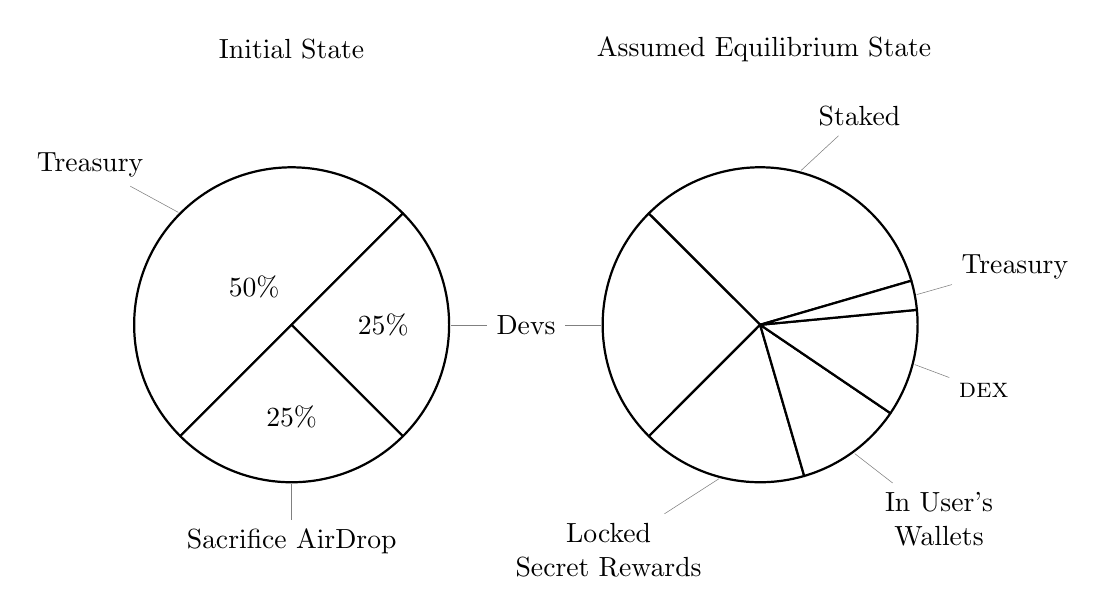
\begin{tikzpicture}[align=center]

\node at (0,3.5) {Initial State};

\pie[color=white,pos={0,0},radius=2,rotate=45,text=pin]{
	50/Treasury,
    25/Sacrifice AirDrop,
    25/Devs};

\node at (6,3.5) {Assumed Equilibrium State};
\pie[hide number,color=white,pos={5.95,0},radius=2,rotate=16.25,text=pin]{
    33/Staked,
	25/\phantom{Devs},
	17/Locked\\Secret Rewards,
	11/In User's\\Wallets,
	11/\textsc{dex},
	3/Treasury};

\end{tikzpicture}
\end{center}

\end{document}

% vim: fdm=marker fmr=<<<,>>>
